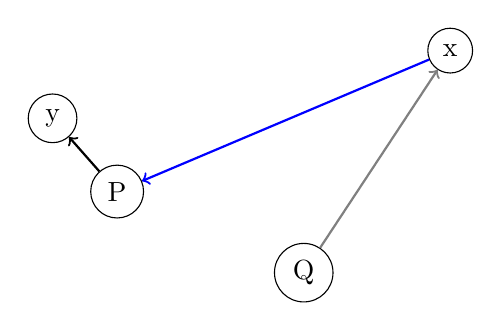
\begin{tikzpicture}
\node[circle, draw=black] (a) at (2.92, -4.38) {Q};
\node[circle, draw=black] (b) at (4.78, -1.56) {x};
\node[circle, draw=black] (c) at (0.55, -3.35) {P};
\node[circle, draw=black] (d) at (-0.27, -2.42) {y};
\draw[->, thick, gray] (a) -- (b);
\draw[->, thick, blue] (b) -- (c);
\draw[->, thick, black] (c) -- (d);
\end{tikzpicture}